\documentclass[11pt,a4paper]{ctexart}

\usepackage{geometry}
\geometry{left=2.2cm,right=2.2cm,top=2.4cm,bottom=2.4cm}
\usepackage{amsmath,amssymb}
\usepackage{graphicx}
\usepackage{booktabs}
\usepackage{longtable}
\usepackage{array}
\usepackage{tabularx}
\usepackage{multirow}
\usepackage{caption}
\usepackage{float}
\usepackage{enumitem}
\usepackage{xcolor}
\usepackage{hyperref}
\usepackage{fancyhdr}
\usepackage{listings}

\graphicspath{{figures/}}
\hypersetup{colorlinks=true,linkcolor=black,urlcolor=blue!50!black}
\captionsetup{font=small,labelfont=bf}
\setlist{itemsep=2pt,topsep=3pt,parsep=0pt}
\renewcommand{\arraystretch}{1.25}

\pagestyle{fancy}
\fancyhf{}
\fancyhead[L]{\small SHYL-WJ86 实验箱在线模拟}
\fancyhead[R]{\small 使用说明}
\fancyfoot[C]{\small \thepage}
\renewcommand{\headrulewidth}{0.4pt}

\lstset{
  basicstyle=\ttfamily\small,
  columns=fullflexible,
  frame=single,
  framerule=0.3pt,
  rulecolor=\color{black!30},
  backgroundcolor=\color{black!3},
  breaklines=true,
  showstringspaces=false
}

\title{\bfseries SHYL-WJ86 微机原理接口实验箱\\[2pt] 在线模拟 · 使用说明}
\author{}
\date{2026 年 11 月}

\begin{document}

\begin{titlepage}
\centering
\vspace*{3cm}
{\LARGE\bfseries SHYL-WJ86 微机原理接口实验箱}\\[6pt]
{\LARGE\bfseries 在线模拟 · 使用说明}\\[18pt]
{\large 8086 实模式 \quad 8253 / 8255 / 8259 / DAC0832 / ADC0809}\\[10pt]
{\large 8 位数码管 \quad 8 位 LED \quad 8$\times$8 点阵 \quad 虚拟示波器}\\[40pt]
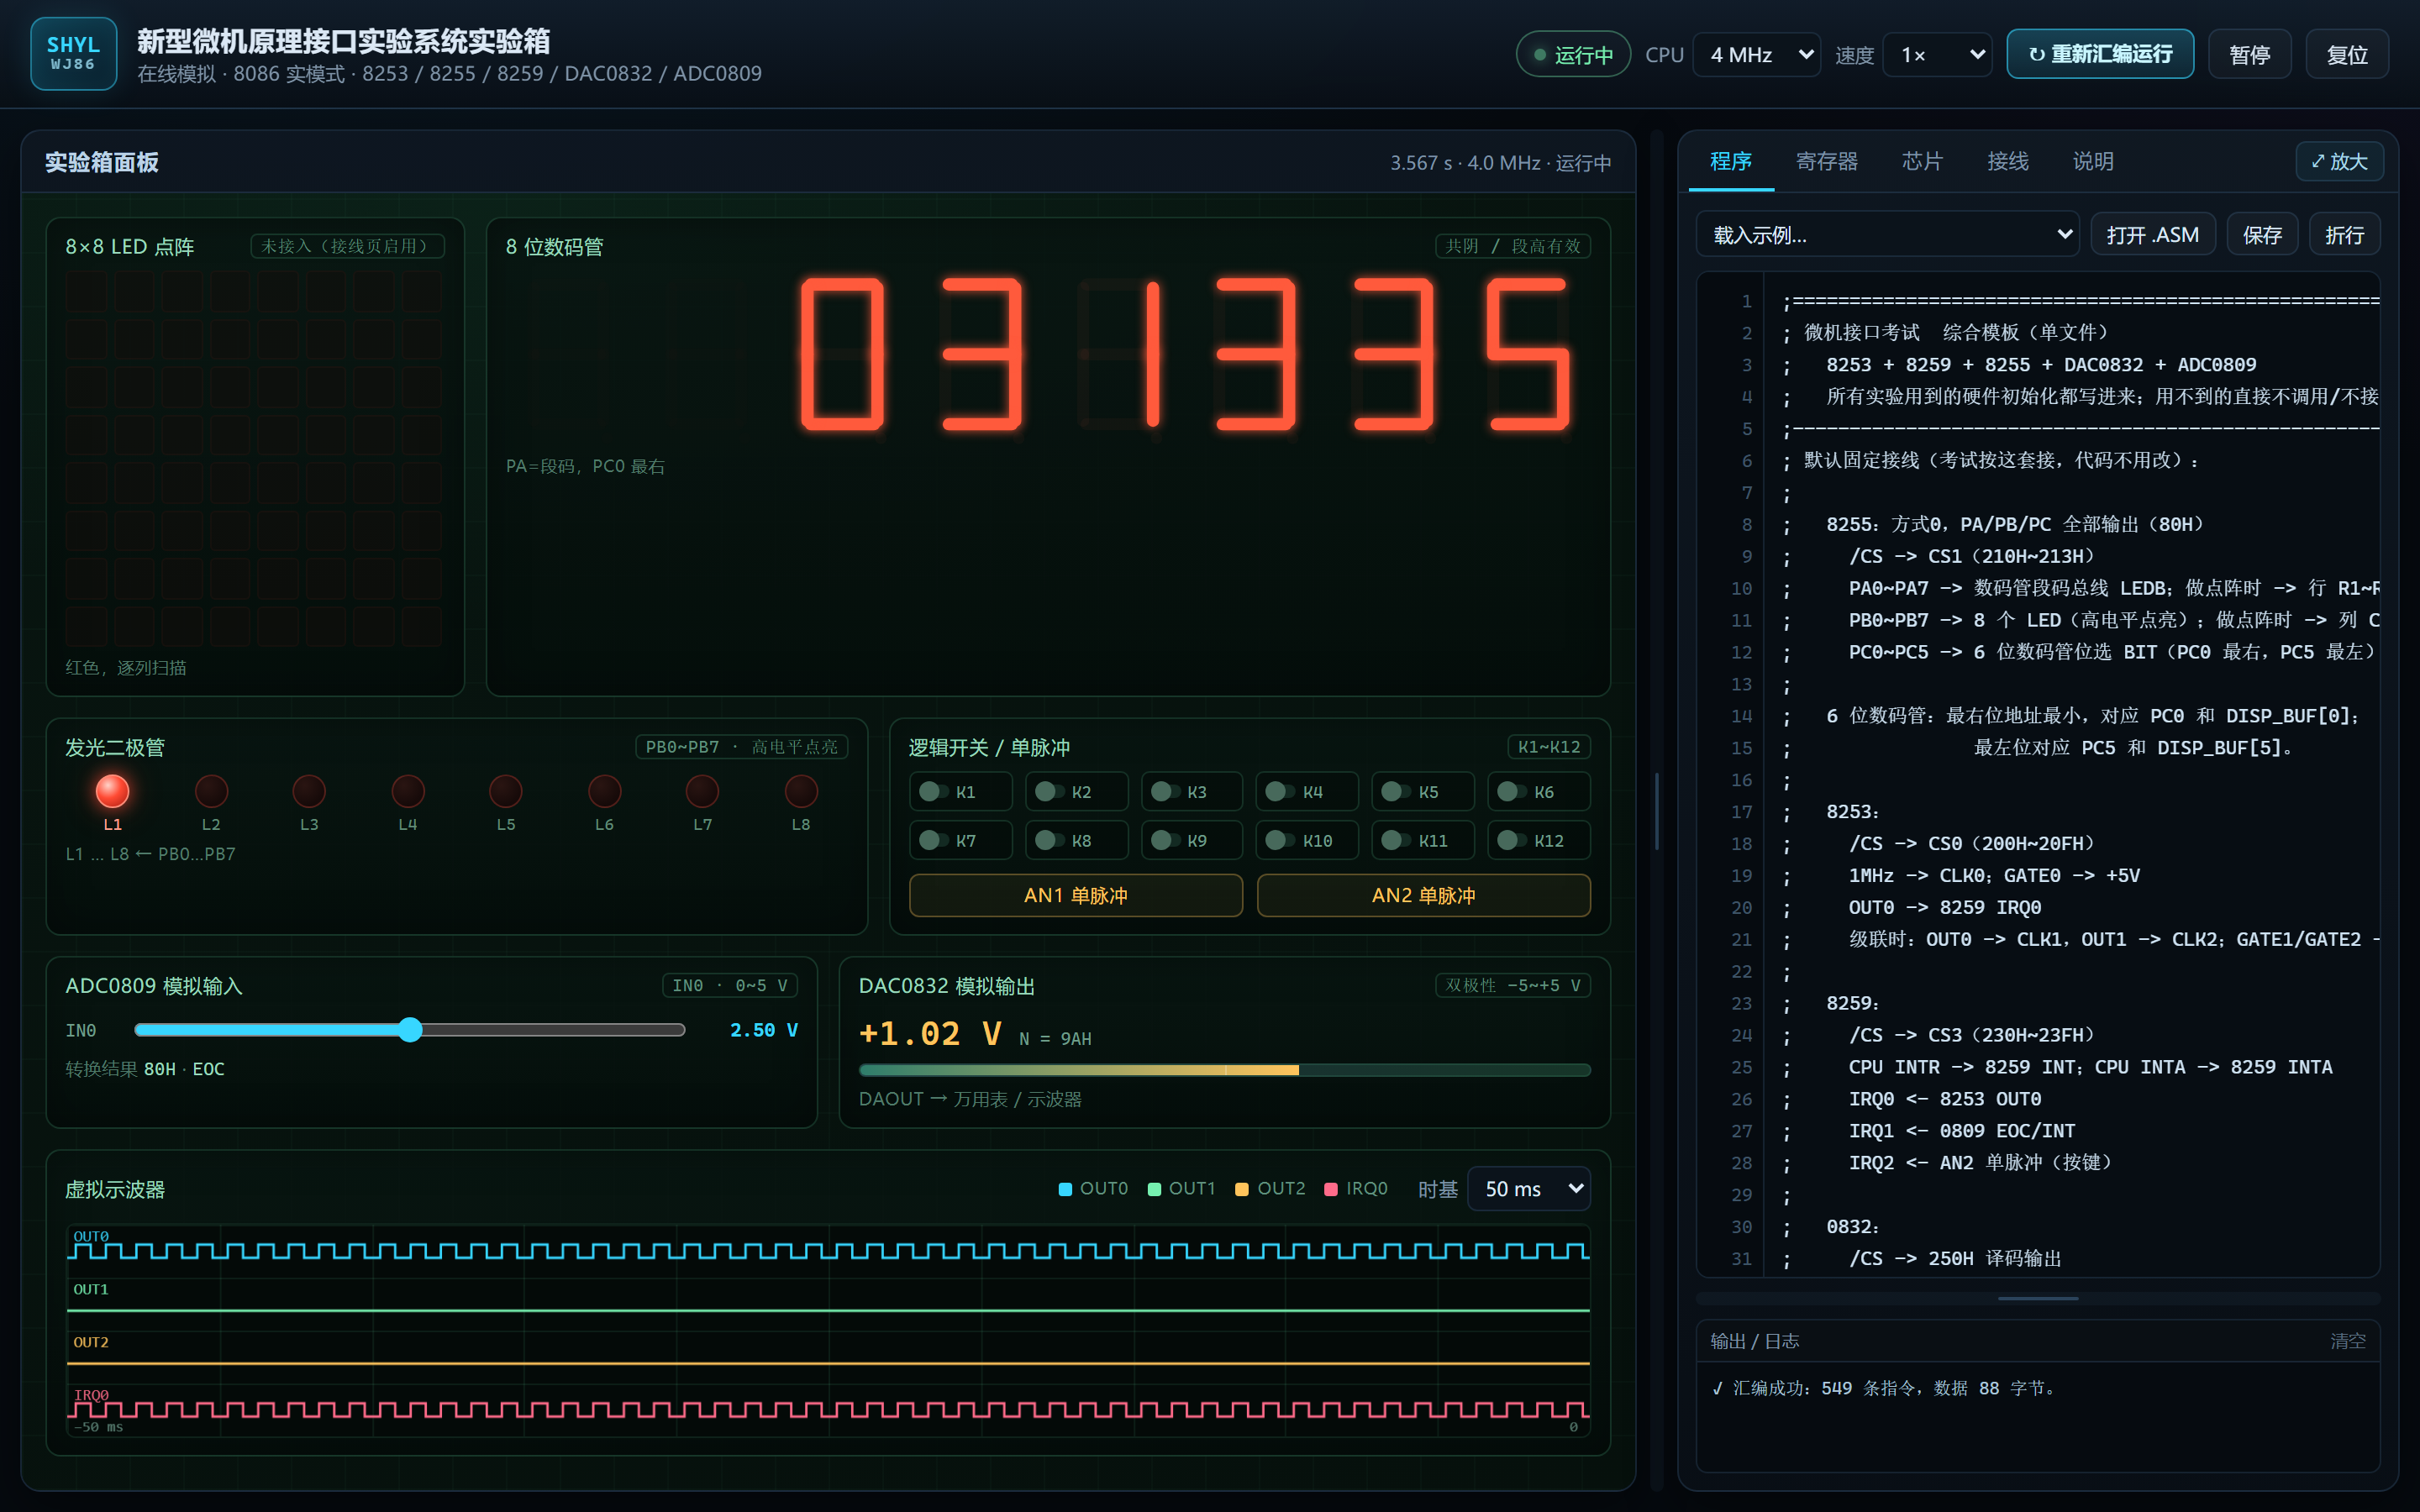
\includegraphics[width=0.86\textwidth]{fig01_exam.png}\\[12pt]
{\small 图：模拟器主界面（考试综合模板运行 3.4 s）}\\[30pt]
{\large 2026 年 11 月}
\vfill
{\small 本说明随模拟器一起交付，离线可用；双击 \texttt{index.html} 即可启动。}
\end{titlepage}

\tableofcontents
\newpage

\section{软件概述}

本软件是一个运行在浏览器中的 SHYL-WJ86 新型微机原理接口实验系统实验箱模拟器。
它用 JavaScript 实现 8086 实模式指令解释器、MASM 子集汇编器，以及 8253/8254、
8255、8259、DAC0832、ADC0809 的行为模型，并把实验箱面板上的数码管、LED、点阵、
开关、单脉冲按钮和示波器绘制在网页上。

使用时不需要安装开发环境，也不需要连接实验箱：双击 \texttt{index.html} 即可打开，
载入或粘贴实验代码，点“汇编并运行”，就能观察程序在面板上的现象。软件完全离线运行，
不依赖网络和外部字体。

主要功能如下：

\begin{itemize}
  \item 直接运行实验指导书中的 \texttt{.ASM} 文件，支持 UTF-8 与 GBK/GB18030 编码；
  \item 实时显示 8 位数码管、8 个 LED、8$\times$8 点阵、开关量和单脉冲；
  \item 模拟 8253 的六种工作方式、级联和 GATE 门控；
  \item 模拟 8259 的 ICW/OCW 初始化、边沿触发、优先级和 EOI；
  \item 模拟 0809 的通道选择、100 $\mu$s 转换、EOC/INT 与中断方式读数；
  \item 模拟 0832 的双极性输出，并用虚拟万用表和示波器显示；
  \item 可调 CPU 主频（2/4/8/16/33 MHz）与仿真倍速（0.25$\times$~4$\times$）。
\end{itemize}

\section{运行环境与启动}

\subsection{运行环境}

推荐使用 Windows 10/11 上的 Chrome 或 Edge（Chromium 内核，版本 100 以上）。
Firefox 亦可运行；不支持 IE。页面使用普通 \texttt{<script>} 加载脚本，因此可以直接以
\texttt{file://} 方式打开，不需要本地服务器。

\subsection{启动步骤}

\begin{enumerate}
  \item 解压交付目录，保持 \texttt{index.html}、\texttt{css/}、\texttt{js/} 的相对位置不变。
  \item 双击 \texttt{index.html}。页面会自动载入“考试综合模板”并开始运行。
  \item 在“程序”页粘贴代码，或点“打开 .ASM”选择文件，然后点右上角“汇编并运行”
        （快捷键 \texttt{Ctrl+Enter}）。
  \item 需要观察某个实验时，在“载入示例”下拉框中选择对应例程；模拟器会自动套用该例程
        所需的接线。
\end{enumerate}

\section{界面与操作}

\subsection{实验箱面板}

主界面左侧是实验箱面板，自上而下依次为：

\begin{itemize}
  \item \textbf{8$\times$8 LED 点阵}：PA 送行数据（PA7 为最上一行），PB 送列选通
        （PB0 为最左一列）。勾选“点阵接法”后显示红色点阵。
  \item \textbf{8 位数码管}：PA0$\sim$PA7 为段码 a$\sim$g、dp，PC0$\sim$PC7（或 PB0$\sim$PB7）
        为位选；按扫描余辉模型显示。
  \item \textbf{发光二极管}：默认 PB0$\sim$PB7 对应 L1$\sim$L8，高电平点亮；
        可改为 PA 输出（交通灯实验）。
  \item \textbf{逻辑开关与单脉冲}：K1$\sim$K12 可点击切换 0/1；AN1、AN2 为单脉冲按钮。
  \item \textbf{ADC0809 模拟输入}：拖动 IN0 滑块设置 0$\sim$5 V 输入电压。
  \item \textbf{DAC0832 模拟输出}：显示当前数字量 N 与双极性输出电压。
  \item \textbf{虚拟示波器}：显示 OUT0、OUT1、OUT2 与 IRQ0 的波形，时基可选
        1 ms$\sim$5 s。
\end{itemize}

\subsection{右侧工作区}

右侧有五个标签页：

\begin{description}[leftmargin=2.2em]
  \item[程序] 汇编代码编辑区、内置示例、打开/保存、汇编错误列表、输出日志。
  \item[寄存器] AX$\sim$SS、IP、周期计数与 CF/PF/AF/ZF/SF/TF/IF/DF/OF 标志。
  \item[芯片] 8253 三个通道、8255 三个端口、8259 的 IMR/IRR/ISR、0809 与 0832 状态。
  \item[接线] 自由接线表：CLK、GATE、IRQ、PC 输入、LED 源，以及显示极性与位序。
  \item[说明] 快速上手、端口表、位序说明和快捷键。
\end{description}

\subsection{运行控制}

\begin{itemize}
  \item \textbf{汇编并运行}：重新汇编当前编辑区内容，成功后从入口开始运行。
  \item \textbf{暂停/继续}：冻结 CPU 与芯片时间，面板保持当前状态。
  \item \textbf{复位}：CPU、内存、芯片和虚拟时间回到初始状态，程序和接线保留。
  \item \textbf{CPU 主频}：改变指令执行速度；8253 的 1 MHz 时钟不受影响。
  \item \textbf{速度}：整机仿真倍速，只影响墙钟时间，不改变程序逻辑。
\end{itemize}

\begin{figure}[H]
  \centering
  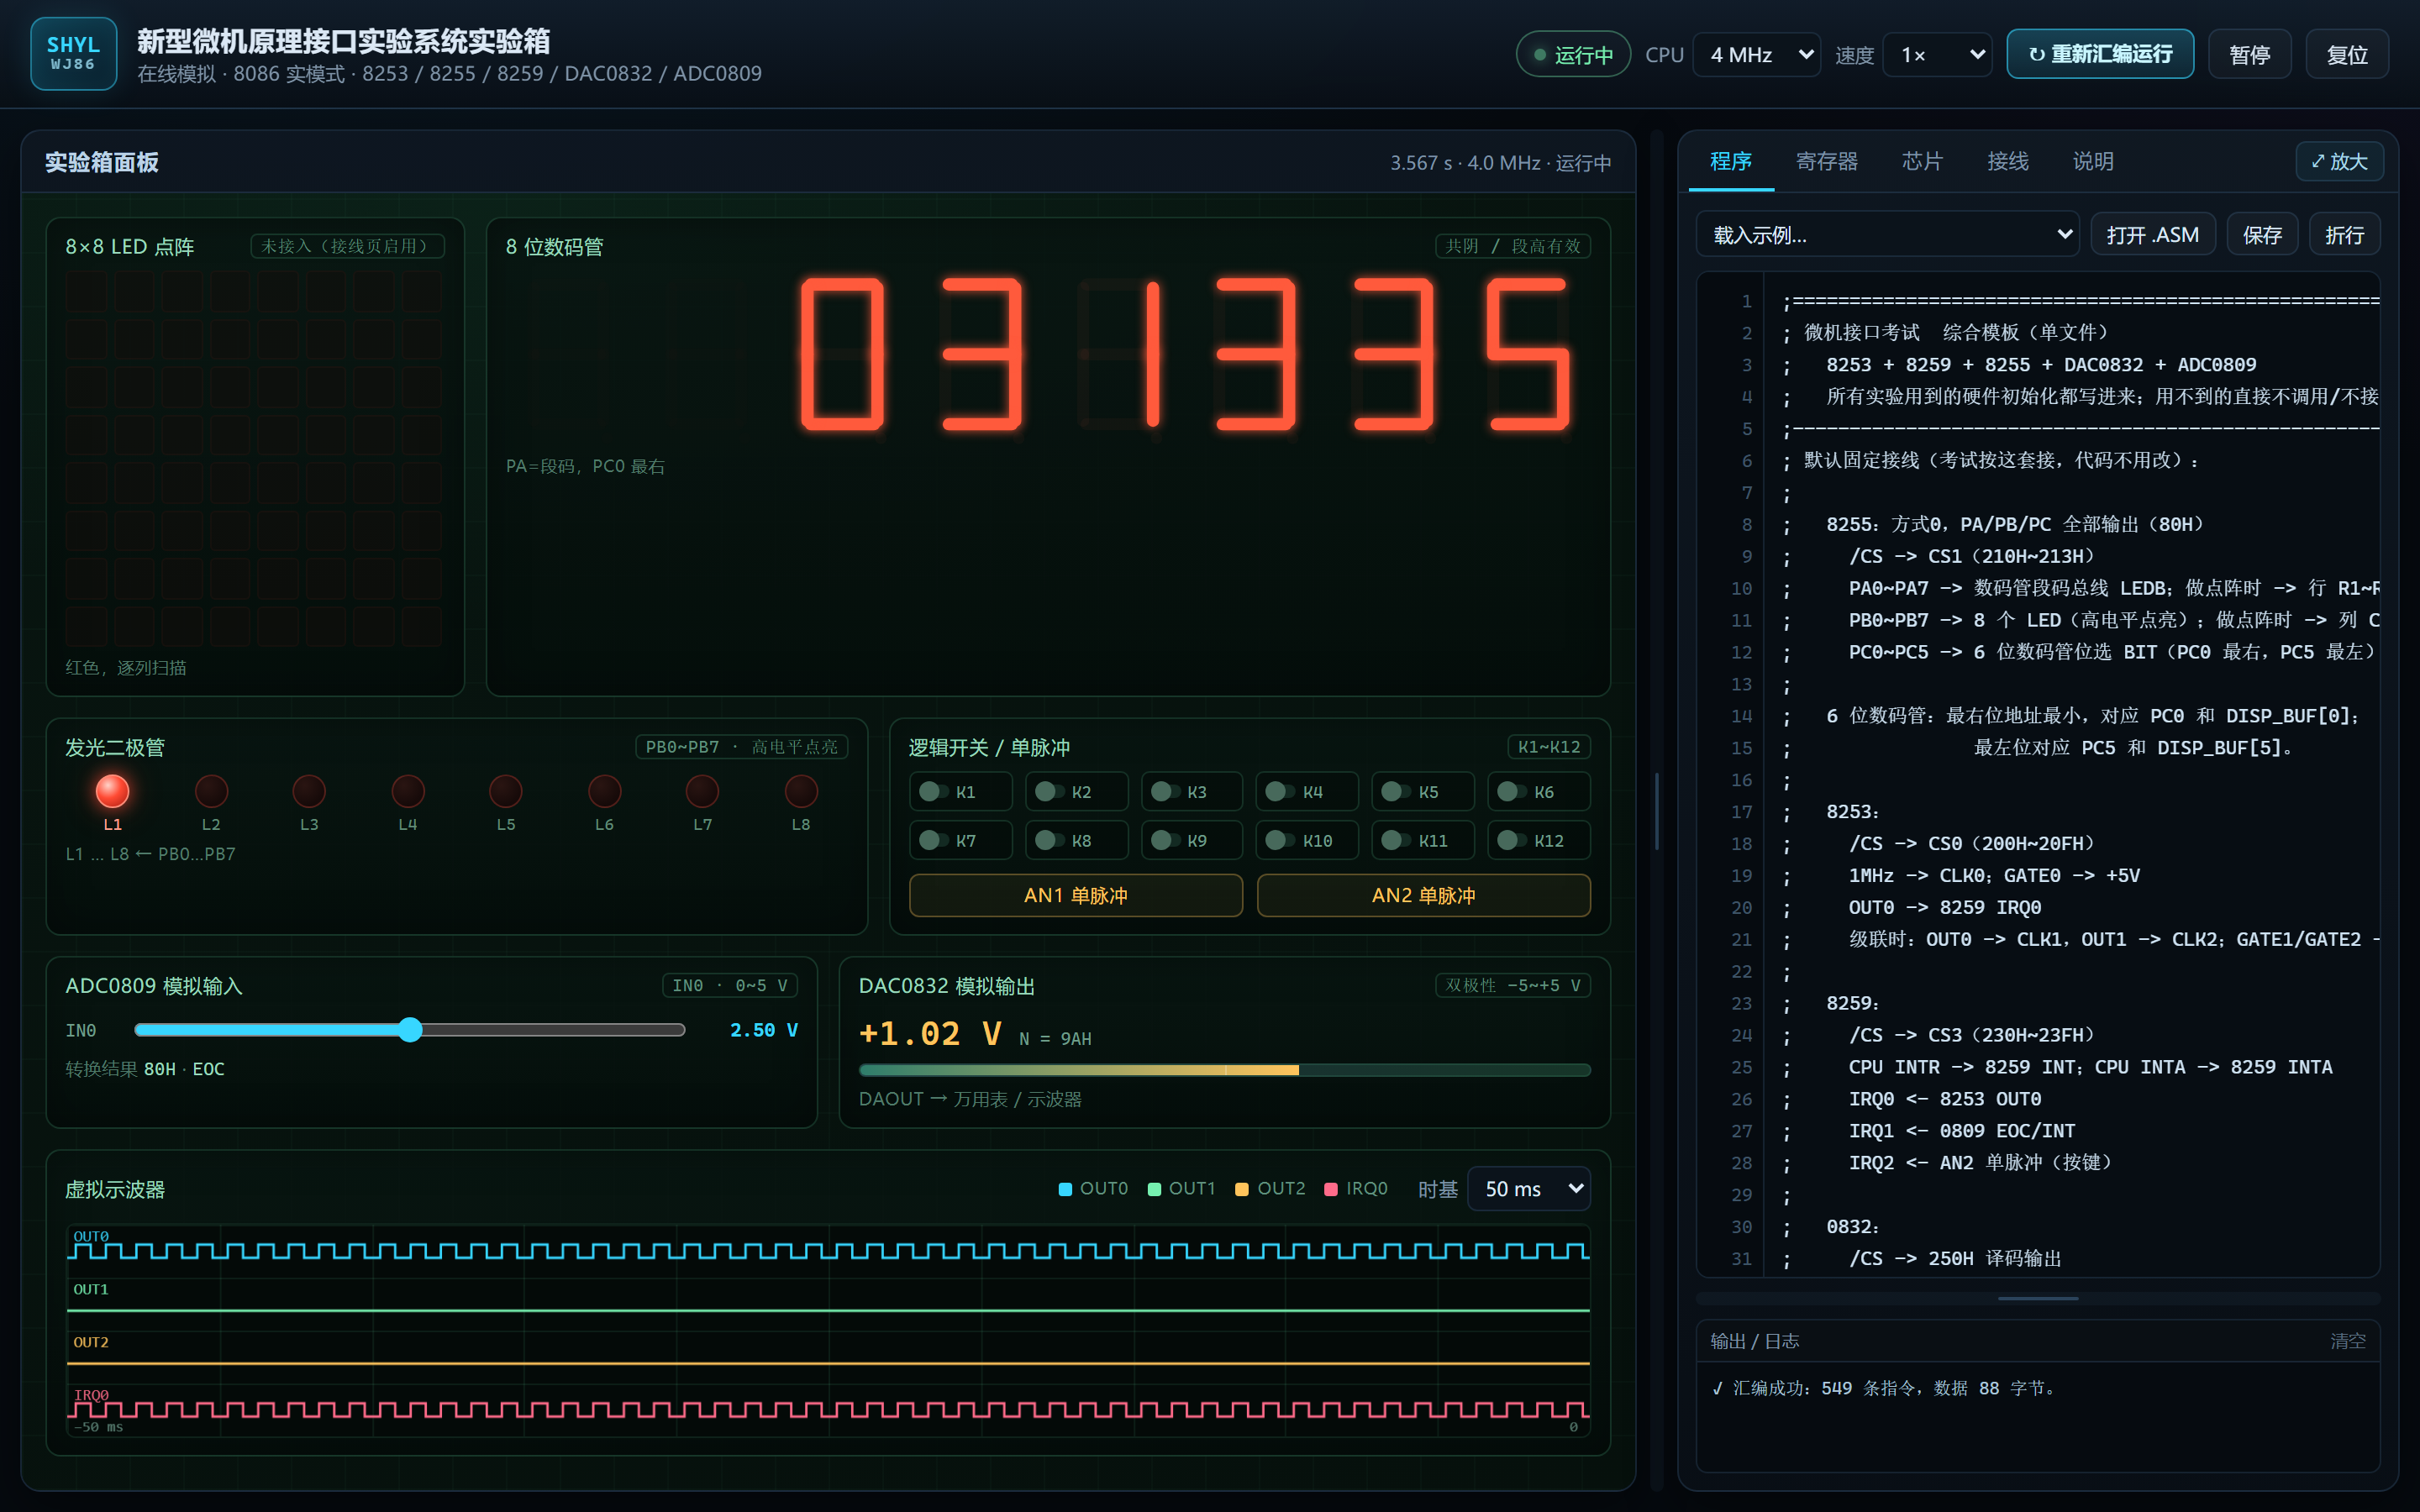
\includegraphics[width=0.96\textwidth]{fig01_exam.png}
  \caption{主界面：考试综合模板运行 3.4 s 时的面板与代码区}
  \label{fig:main}
\end{figure}

\begin{figure}[H]
  \centering
  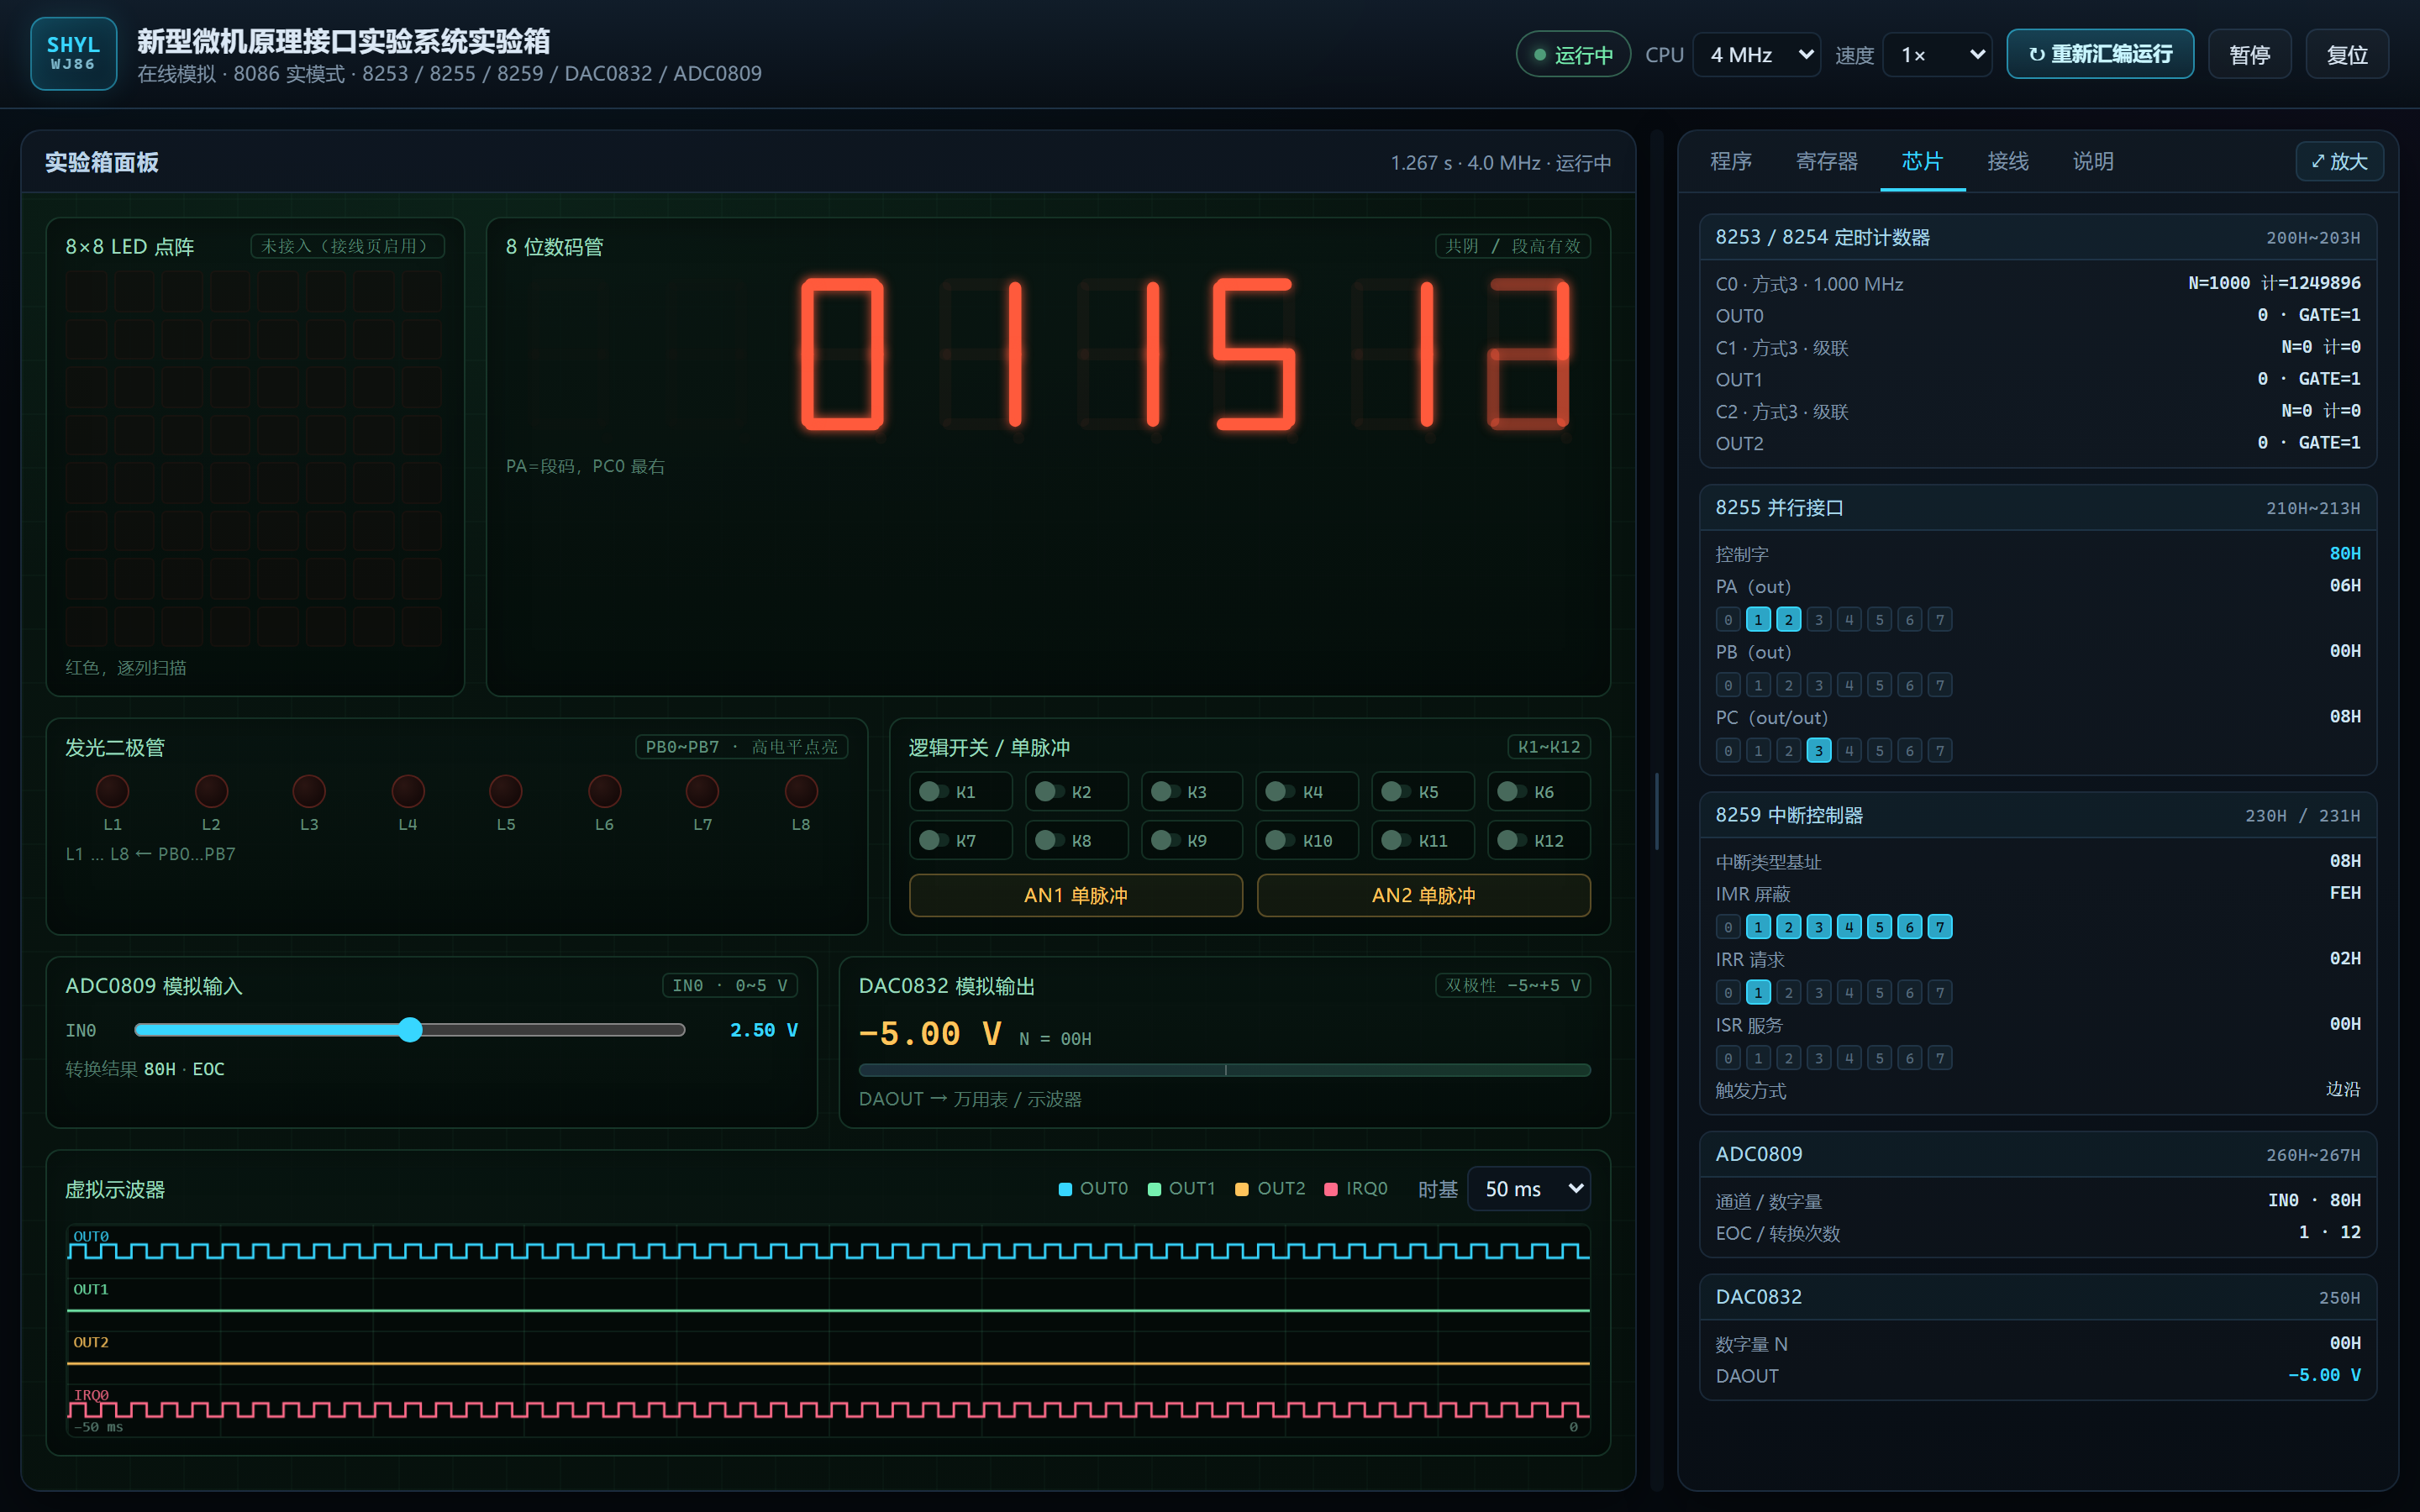
\includegraphics[width=0.96\textwidth]{fig04_chips.png}
  \caption{“芯片”页：8253 计数、8255 端口、8259 的 IMR/IRR/ISR 以及 0809/0832 状态}
  \label{fig:chips}
\end{figure}

\section{内置示例与现象}

“载入示例”中包含八个常用实验，均已配置好接线。选择后模拟器会自动汇编并运行。

\begin{longtable}{>{\raggedright\arraybackslash}p{3.3cm} >{\raggedright\arraybackslash}p{6.8cm} >{\raggedright\arraybackslash}p{5.0cm}}
\toprule
示例 & 观察到的现象 & 关键接线 \\
\midrule
\endhead
考试综合模板 & 数码管显示 BBCCDD（如 3.3 s 时为 03 13 33）；LED 每 2 秒多亮一个；DAC 每 2 秒换一档电压 & 默认接线 \\
实验三-1：8253 计脉冲 & 按 AN1 十次后 OUT0 变高，L1 点亮 & CLK0$\leftarrow$AN1；OUT0$\rightarrow$L1 \\
实验三-2：2 秒方波 & L1 亮 1 秒、灭 1 秒 & OUT0$\rightarrow$CLK1；OUT1$\rightarrow$L1 \\
实验五-1：8259 按键中断 & 每按一次 AN2，数码管加 1，9 后回 0 & 默认接线（IRQ2$\leftarrow$AN2） \\
实验四-1：DAC 五档电压 & 1.0、2.0、3.0、4.0、4.5 V 循环，每档保持 2 秒 & OUT0$\rightarrow$PC7（1 ms 节拍） \\
实验四-3：ADC 十六进制 & 拖动 IN0，最右两位显示 00$\sim$FF；2.50 V 对应 80H & OUT0$\rightarrow$PC7；位选接 PB \\
实验三-6：8$\times$8 点阵 & 红色循环显示“接口技术”，每字 1.8 秒 & OUT0$\rightarrow$PC7；点阵接法 \\
实验三-5：8253 交通灯 & PA0$\sim$PA5 按绿 10 秒、黄 2 秒、红/绿交换循环 & OUT0$\rightarrow$CLK1；OUT1$\rightarrow$PC0；LED 接 PA \\
\bottomrule
\end{longtable}

\begin{figure}[H]
  \centering
  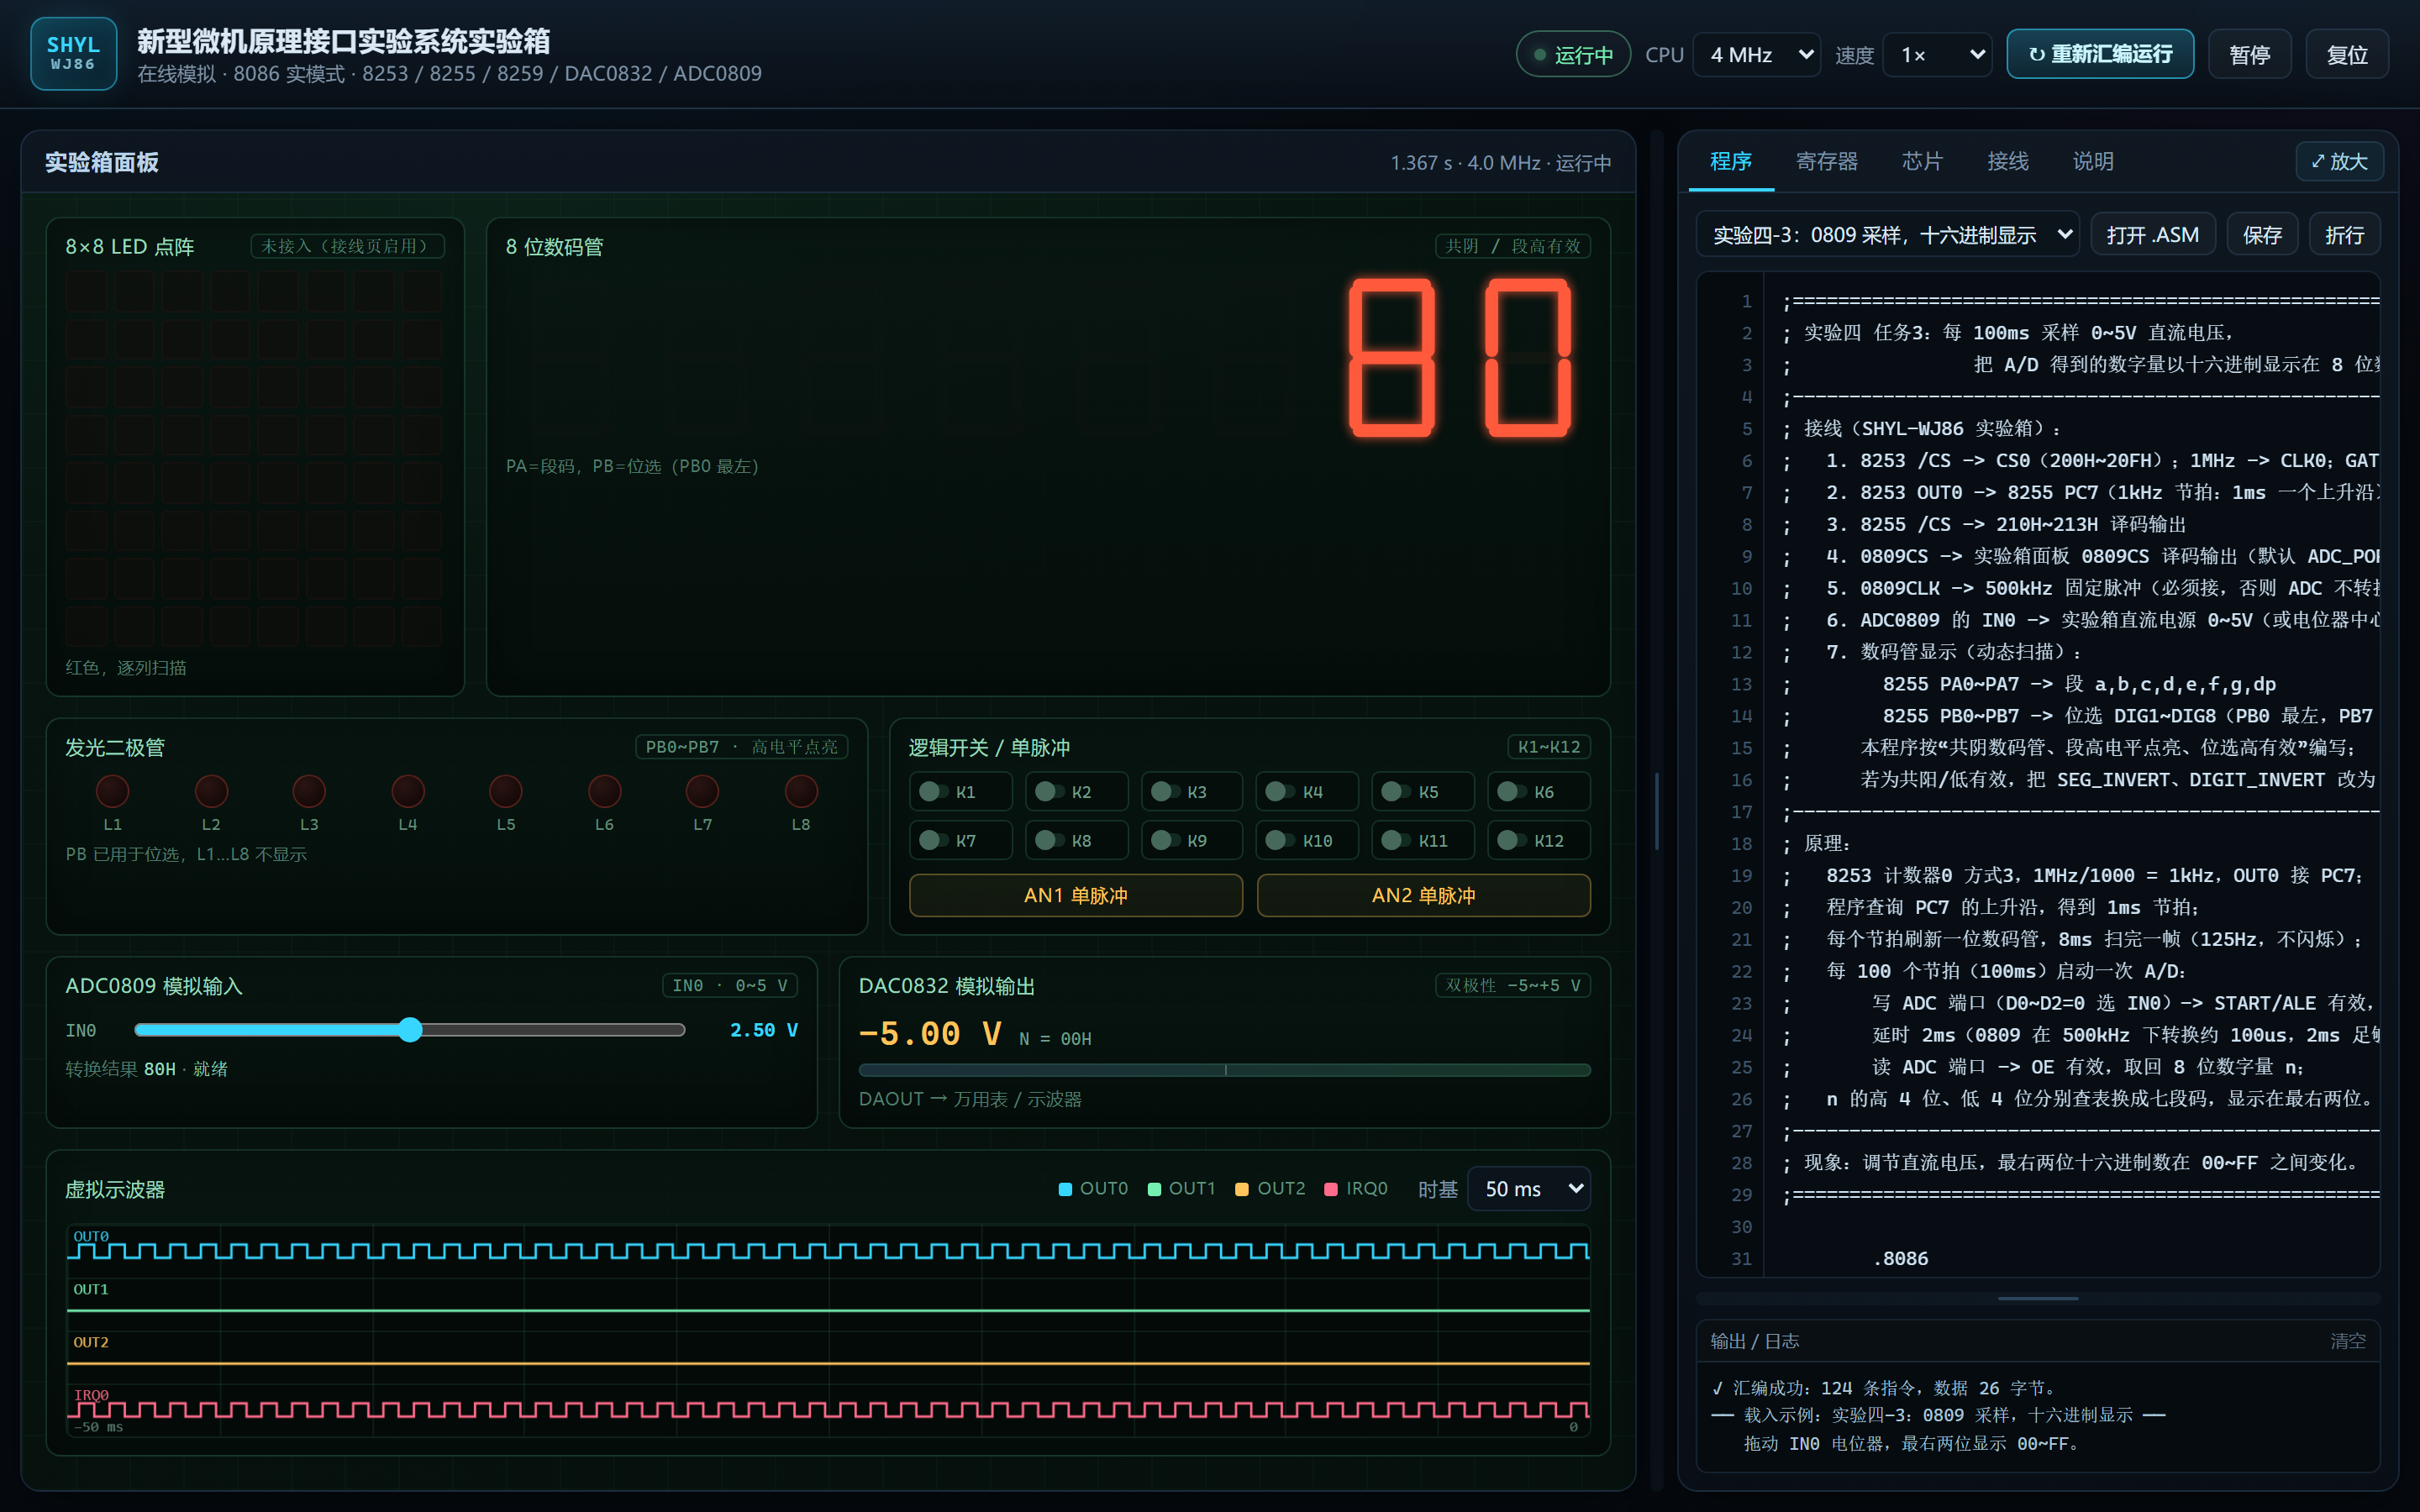
\includegraphics[width=0.96\textwidth]{fig02_adc.png}
  \caption{实验四-3：IN0 = 2.50 V 时，最右两位数码管显示 80H}
  \label{fig:adc}
\end{figure}

\begin{figure}[H]
  \centering
  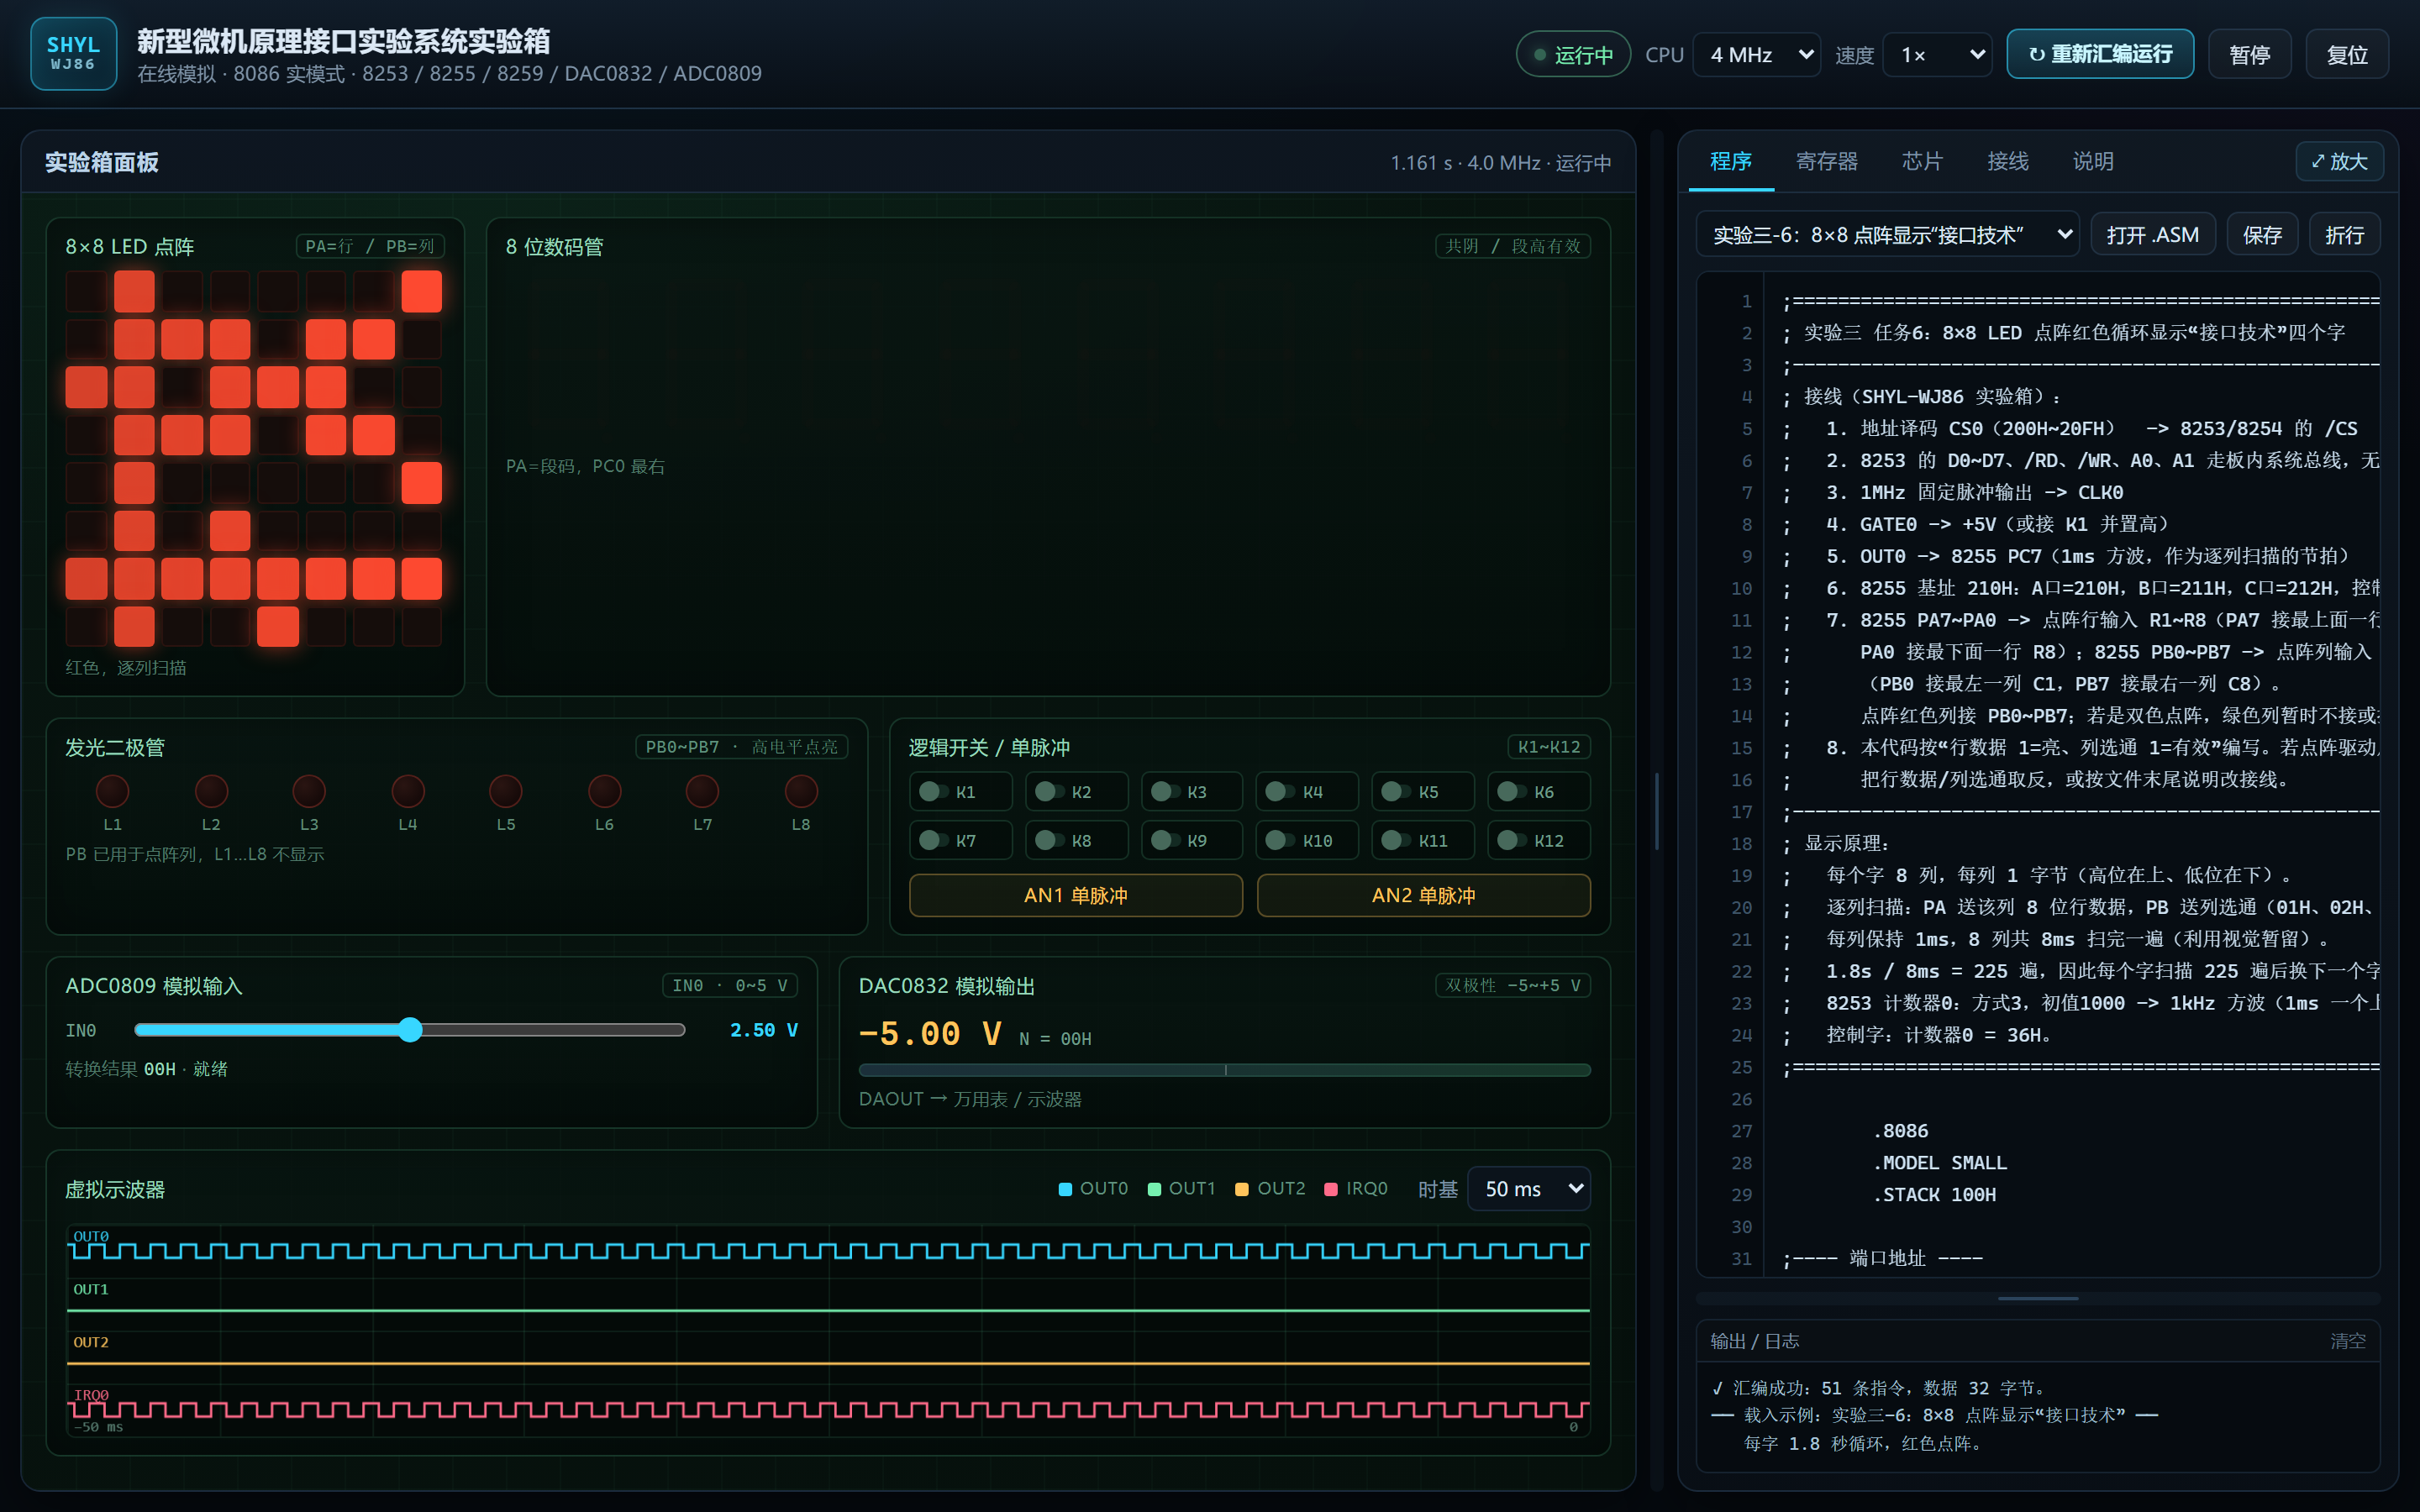
\includegraphics[width=0.96\textwidth]{fig03_matrix.png}
  \caption{实验三-6：8$\times$8 点阵显示“接口技术”的第一个字“接”}
  \label{fig:matrix}
\end{figure}

\section{接线与端口}

\subsection{端口地址}

\begin{table}[H]
\centering
\small
\begin{tabularx}{0.92\textwidth}{>{\ttfamily}l l X}
\toprule
端口 & 器件 & 说明 \\
\midrule
200H$\sim$202H & 8253 & 计数器 0/1/2 \\
203H & 8253 & 控制字寄存器 \\
210H$\sim$212H & 8255 & PA/PB/PC \\
213H & 8255 & 控制字寄存器 \\
230H/231H & 8259 & 偶地址 ICW1/OCW2/OCW3，奇地址 ICW2$\sim$4/OCW1 \\
250H & DAC0832 & 写数字量 N \\
260H$\sim$267H & ADC0809 & 写启动（D0$\sim$D2 选通道），读结果 \\
\bottomrule
\end{tabularx}
\caption{实验箱端口分配}
\end{table}

\subsection{默认接线}

\begin{itemize}
  \item 8253：1 MHz 固定脉冲$\rightarrow$CLK0；GATE0$\sim$GATE2 接 +5 V；
        OUT0$\rightarrow$8259 IRQ0。
  \item 8255：PA 接数码管段码 / 点阵行；PB 接 8 个 LED / 点阵列；PC 接数码管位选。
  \item 8259：0809 的 EOC/INT$\rightarrow$IRQ1；AN2 单脉冲$\rightarrow$IRQ2；
        CPU 的 INTR/INTA 与 8259 对应相连。
  \item 0832：片选 250H；Uref = +5 V；DAOUT 接万用表或示波器。
  \item 0809：片选 260H；CLK 接 500 kHz；IN0 接 0$\sim$5 V 电位器。
\end{itemize}

\subsection{自由接线}

“接线”页是一张自由接线表：每个目的端在左侧，右侧下拉框选择信号源；同一信号可以同时接到多路。

\begin{itemize}
  \item \texttt{CLK0}$\sim$\texttt{CLK2}：固定脉冲（1 MHz、500 kHz、100 kHz、10 kHz、1 kHz、
        100 Hz、10 Hz、1 Hz）、\texttt{OUT0}$\sim$\texttt{OUT2}、\texttt{AN1}、\texttt{K1}$\sim$\texttt{K12}、\texttt{GND}；
  \item \texttt{GATE0}$\sim$\texttt{GATE2}：\texttt{+5V}、\texttt{GND}、\texttt{OUT0}$\sim$\texttt{OUT2}、
        \texttt{AN1}、\texttt{AN2}、\texttt{K1}$\sim$\texttt{K12}；
  \item \texttt{IRQ0}$\sim$\texttt{IRQ7}：\texttt{OUT0}$\sim$\texttt{OUT2}、\texttt{EOC}、
        \texttt{AN1}、\texttt{AN2}、\texttt{K1}$\sim$\texttt{K12}、\texttt{+5V}、\texttt{GND}、\texttt{NC}；
  \item \texttt{PC0}$\sim$\texttt{PC7}：\texttt{OUT0}$\sim$\texttt{OUT2}、\texttt{EOC}、
        \texttt{AN1}、\texttt{AN2}、\texttt{K1}$\sim$\texttt{K12}、\texttt{+5V}、\texttt{GND}；
  \item \texttt{L1}$\sim$\texttt{L8}：\texttt{PB0}$\sim$\texttt{PB7}、\texttt{PA0}$\sim$\texttt{PA7}、
        \texttt{OUT0}$\sim$\texttt{OUT2}、\texttt{AN1}、\texttt{AN2}、\texttt{K1}$\sim$\texttt{K12}、
        \texttt{+5V}、\texttt{GND}、\texttt{NC}。
\end{itemize}

此外，8255 的 \texttt{PA0}$\sim$\texttt{PA7}、\texttt{PB0}$\sim$\texttt{PB7}、\texttt{PC0}$\sim$\texttt{PC7}
引脚也可以作为任意一路的源。

“默认接线”“8253 级联”“1 ms 节拍$\rightarrow$PC7”“点阵接线”“交通灯”五个按钮可以快速套用常用组合。
显示部分另有数码管位选端口（PC/PB）、点阵接法、共阳/共阴、位选极性与 LED 极性。

修改接线立即生效；复位后保留。若把某根线改到与程序不符的位置，面板会显示对应错误现象，
可对照“芯片”页的端口值排查。

\begin{figure}[H]
  \centering
  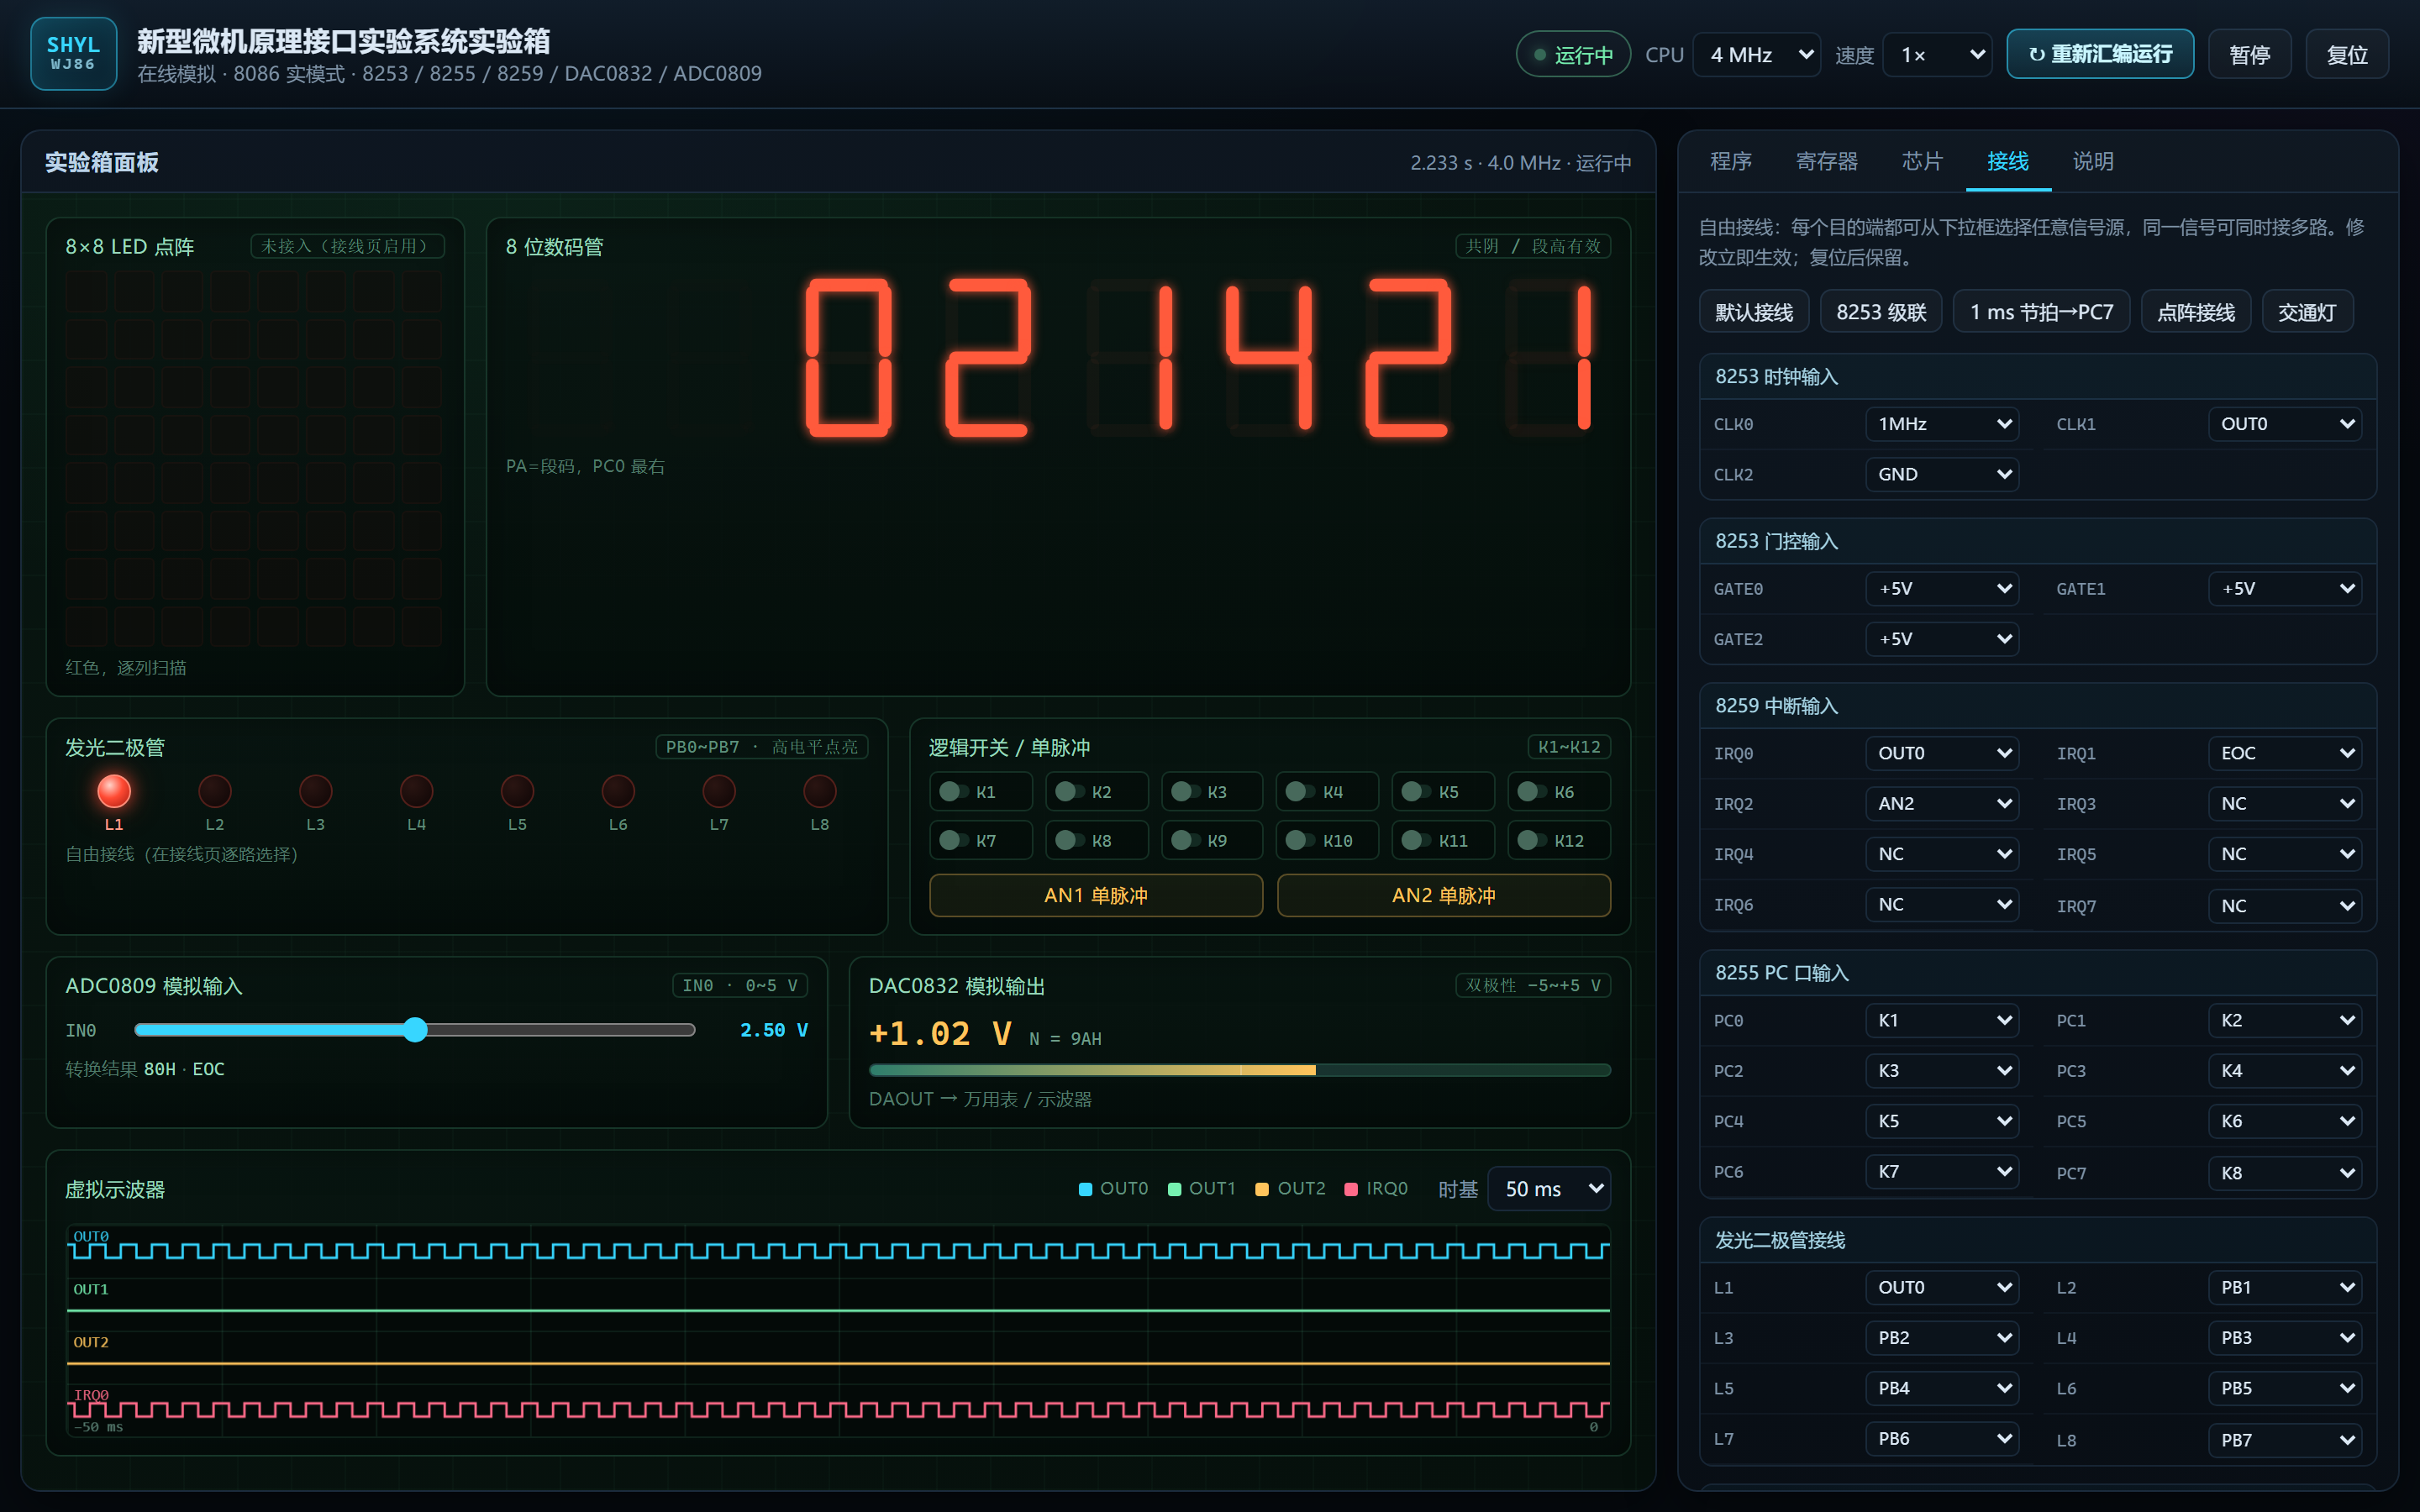
\includegraphics[width=0.96\textwidth]{fig05_wire.png}
  \caption{接线页：自由接线表、常用预设与显示极性}
  \label{fig:wire}
\end{figure}

\section{数码管位序、极性与点阵}

\subsection{位序}

实验代码对数码管位序的约定并不统一：

\begin{itemize}
  \item 考试综合模板按 \textbf{PC0 最右} 编写，即 PC0 选最右一位，显示缓冲下标 0 对应最右位；
  \item 实验四、实验五的多数例程按 \textbf{PC0 最左} 编写，显示缓冲下标 0 对应最左位；
  \item 实验四-3 用 \textbf{PB} 做位选（PB0 最左）。
\end{itemize}

模拟器默认采用 PC0 最右。若载入手写代码后发现显示左右颠倒，到“接线”页勾选
“数码管位序反转（PC0 最左）”，或把“数码管位选端口”改为 PB。内置示例已按各自代码
设置好位序。

\subsection{极性}

\begin{itemize}
  \item 段码极性：共阴数码管段高有效，共阳数码管段低有效；对应“共阳数码管（段码反相）”。
  \item 位选极性：多数模块位选高有效；若模块低有效，勾选“位选低有效”。
  \item LED 极性：默认高电平点亮；低电平点亮的模块勾选“LED 低电平点亮”。
\end{itemize}

\subsection{点阵}

点阵按“PA 行、PB 列”接法：PA7 为最上一行，PB0 为最左一列，行/列均为高有效。
未勾选“点阵接法”时，PA/PB 仍按数码管段码和 LED 解释，点阵区域显示为未接入。
若点阵模块行或列反相，勾选对应的“行反相 / 列反相”。

\section{汇编器与 CPU}

\subsection{支持范围}

汇编器按 MASM 常用子集实现，支持：

\begin{itemize}
  \item 伪指令：\texttt{.8086}、\texttt{.386}、\texttt{.486}、\texttt{.MODEL SMALL}、
        \texttt{.STACK}、\texttt{.DATA}、\texttt{.CODE}、\texttt{NAME SEGMENT/ENDS}、
        \texttt{ASSUME}、\texttt{PROC/ENDP}、\texttt{EQU}、\texttt{DB/DW/DD}、
        \texttt{DUP}、\texttt{END}；
  \item 数据：字节、字、字符串、\texttt{?}、\texttt{DUP}、\texttt{OFFSET}、\texttt{SEG}；
  \item 指令：8086 常用整数指令，包括数据传送、算术、逻辑、移位/循环移位、转移、
        循环、子程序、中断、I/O、串操作与 \texttt{REP} 前缀；
  \item \texttt{INT 21H} 的 09H（显示字符串）、02H（显示字符）、4CH（结束）。
\end{itemize}

不支持 32 位寄存器与指令、保护模式、宏、外部符号链接；代码地址是“指令序号”而不是
字节偏移，因此 \texttt{\$} 和依赖指令长度的技巧不精确。

\subsection{时间模型}

CPU 默认 4 MHz，每条指令按大约 4$\sim$30 个时钟周期折算；8253 的输入时钟按实际频率
推进，0809 每次转换 100 $\mu$s，8259 在指令边界采样中断请求并在 \texttt{IF=1} 时响应。
CPU 主频可在右上角切换；改变主频会改变软件延时循环的绝对时间，但不改变 8253 的定时。

\section{常见问题}

\begin{description}[leftmargin=2.2em]
  \item[数码管全灭] 检查 8255 控制字是否为输出、PA 是否接段码、位选端口是否选对
        （PC 或 PB）、段码/位选极性是否与模块一致。可先载入“数码管自检”类程序。
  \item[显示左右颠倒] 勾选“数码管位序反转（PC0 最左）”。
  \item[只亮一位或不亮] 扫描程序可能没有运行，或位选接在另一个端口；观察“芯片”页
        PA/PC（或 PB）是否在快速变化。
  \item[ADC 数值不变] 确认程序向 260H 写过启动字、IN0 滑块有电压、转换后读过结果；
        “芯片”页的“转换次数”应不断增加。
  \item[不进中断] 依次检查：中断向量是否写入、8259 的 IMR 是否放开、ISR 是否发 EOI、
        CPU 是否执行 \texttt{STI}、OUT0/AN2 是否接到对应 IRQ。
  \item[程序跑飞] 控制台会显示“中断向量未安装”“除数为 0”等错误及出错行号；
        修正后重新汇编。
  \item[打开乱码] 模拟器会自动尝试 UTF-8，失败后按 GBK/GB18030 解码；仍乱码时可用
        记事本另存为 UTF-8 再打开。
\end{description}

\section{验证清单}

下表是交付前用无头 Chromium 和 Node 逐项运行得到的结果，可作为使用时的对照。

\begin{longtable}{>{\raggedright\arraybackslash}p{3.6cm} >{\raggedright\arraybackslash}p{5.6cm} >{\raggedright\arraybackslash}p{5.4cm}}
\toprule
程序 & 运行条件 & 结果 \\
\midrule
\endhead
考试模板 & 2.2 s & TICK1MS=2200，B=02、C=14、D=22，LED 1 个，DAC 154（1.02 V） \\
考试模板 & 3.3 s & 数码管 03 13 33 \\
考试模板 + ADC 中断 & IRQ\_MASK=0FCH，IN0=2.5 V & ADC\_VAL=128，显示“U 2.5” \\
考试模板 + 按键中断 & IRQ\_MASK=0FAH，按 AN2 五次 & KEY\_CNT=5 \\
TEST\_DISP & 0.4 s & 8 位数码管依次显示 1$\sim$8 \\
TEST\_IRQ0 & 2.5 s & PB0 每 1 s 翻转一次 \\
实验三-1 & AN1 十个脉冲 & OUT0=1，L1 点亮 \\
实验三-2 & 3 s & OUT1 亮 1 s、灭 1 s \\
实验三-3 & 12 s & OUT2 周期 5 s、低脉冲 1 s \\
实验四-1 & 10 s & N=154、179、205、230、243，每档 2 s \\
实验四-3 & IN0=2.5 V & 数码管 80H \\
实验三-6 & 0.8 s & 点阵显示“接”字，字模 8 列正确 \\
实验三-5 & 14 s & PA=21H（南北红、东西绿），按 10 s/2 s 换相 \\
486 自检 & A86\_486\_TEST2.ASM & 控制台输出“486 OK” \\
\bottomrule
\end{longtable}

\vspace{1em}
\noindent\textbf{说明：}以上结果均在 CPU 4 MHz、仿真倍速 1$\times$（验证脚本部分使用 4$\times$）
下测得；不同主频下软件延时类程序的时间数值会变化，但 8253 定时和中断计数保持一致。

\end{document}

